\documentclass[aip,apl,reprint,twocolumn,superscriptaddress,oneside,floatfix,amsmath,showpacs,amssymb]{revtex4-1}

\usepackage{graphicx}
\usepackage{dcolumn}
\usepackage{bm}
\usepackage[usenames]{color}
\usepackage{tabularx}




\begin{document}

\newcommand{\ie}{\textit{i.e.}}
\newcommand{\eg}{\textit{e.g.}}
\newcommand{\etal}{\textit{et al.}}


%%%%%%%%%%%%%%%%%%%%%%%%%%%% TITLE
\title{Tunable sub-gap radiation detection with Indium Oxide  superconducting resonators}


%%%%%%%%%%%%%%%%%%%%%%%%%%%% AUTHORS

\author{O.~Dupr\'e}
\affiliation{Univ. Grenoble Alpes, Inst NEEL, F-38000 Grenoble, France}
\affiliation{CNRS, Inst NEEL, F-38000 Grenoble, France}

\author{B.~Sac\'ep\'e}
\affiliation{Univ. Grenoble Alpes, Inst NEEL, F-38000 Grenoble, France}
\affiliation{CNRS, Inst NEEL, F-38000 Grenoble, France}

\author{C.~Hoarau}
\affiliation{Univ. Grenoble Alpes, Inst NEEL, F-38000 Grenoble, France}
\affiliation{CNRS, Inst NEEL, F-38000 Grenoble, France}

\author{J.~Goupy}
\affiliation{Univ. Grenoble Alpes, Inst NEEL, F-38000 Grenoble, France}
\affiliation{CNRS, Inst NEEL, F-38000 Grenoble, France}

\author{M.~Calvo}
\affiliation{Univ. Grenoble Alpes, Inst NEEL, F-38000 Grenoble, France}
\affiliation{CNRS, Inst NEEL, F-38000 Grenoble, France}

\author{A.~Beno\^it}
\affiliation{Univ. Grenoble Alpes, Inst NEEL, F-38000 Grenoble, France}
\affiliation{CNRS, Inst NEEL, F-38000 Grenoble, France}

\author{A.~Catalano}
\affiliation{Univ. Grenoble Alpes, Inst NEEL, F-38000 Grenoble, France}
\affiliation{CNRS, Inst NEEL, F-38000 Grenoble, France}

\author{K. Le Calvez}
\affiliation{Univ. Grenoble Alpes, Inst NEEL, F-38000 Grenoble, France}
\affiliation{CNRS, Inst NEEL, F-38000 Grenoble, France}

\author{T.~Klein}
\affiliation{Univ. Grenoble Alpes, Inst NEEL, F-38000 Grenoble, France}
\affiliation{CNRS, Inst NEEL, F-38000 Grenoble, France}

\author{A.~Monfardini}
\affiliation{Univ. Grenoble Alpes, Inst NEEL, F-38000 Grenoble, France}
\affiliation{CNRS, Inst NEEL, F-38000 Grenoble, France}

\author{F.~Levy-Bertrand}
\affiliation{Univ. Grenoble Alpes, Inst NEEL, F-38000 Grenoble, France}
\affiliation{CNRS, Inst NEEL, F-38000 Grenoble, France}

%\date{\today}
%%%%%%%%%%%%%%%%%%%%%%%%%%%% ABSTRACT


\begin{abstract}
We have fabricated Indium Oxide superconductors kinetic inductance detectors that are sensitive to discrete light values of the order of 7 and 14~GHz. Those values ranged far below twice the superconducting gap of the employed Indium Oxyde that worth about 200~GHz. The light detection consists in a shift of the resonance frequency with  no clear change of the quality factor. We demonstrated that the light absorption can be adjusted with the total length of the superconducting resonator. We attributed those observations to surface superconducting plasmons.
\end{abstract}

\pacs{74.25.F-, 74.25.Bt, 74.25.Op, 74.45.+c} 
%PACS 74.	Superconductivity
%PACS 74.25.F-	Properties of superconductors Transport properties
%PACS 74.25.Bt	Properties of superconductors Thermodynamic properties
%PACS 74.25.Op	Properties of superconductors Mixed states, critical fields, and surface sheaths
%PACS 74.45.+c	Properties of superconductors Proximity effects; Andreev reflection; SN and SNS junctions

\maketitle

%\section{Introduction}
Superconducting microwaves resonators are the building blocks of various on going and future technological developments ranging from sensitive photon detectors for astrophysics~\cite{Day}, quantum computation~\cite{Wallraff}, and coupling to nano-electromechanical resonators~\cite{Regal}. The detection principle is based on the monitoring of the resonator frequency variation $\omega_0=(LC)^{-1/2}$. When used as a photon detector, the incident light breaks down Cooper pairs, modifying the kinetic inductance  L  and thus the resonance frequency. The superconducting microwaves resonators are therefore referred as Kinetic Inductance Detector.

The resonator superconducting material directly affects its employability. Indeed, the critical superconducting temperature $T_C$ leads to a temperature usable range  $T<T_C/3$, and the superconducting gap $\Delta$ sets in the photon detector cutoff frequency to $h\nu>2\Delta$. Low superfluid density $n_s$ is anticipated as a key ingredient to reach high sensitivity, potentially up to the detection of a unique photon event, as the relative frequency variation $\delta\omega_0/\omega_0$ is proportional to the superfluid density relative variation $\delta n_S/n_S$. However, in principle, within the classic BCS-superconducting theory  $T_C$, $\Delta$ and $n_S$ are not independent parameters as  $\Delta~=~1.76-2~K_BT_C$ and roughly $T_C\simeq e^{-1/n_S}$. Non-conventional superconductors may offer more flexibility to optimize all the parameters. In that context, we investigated the Indium Oxyde material, InO$_x$, that can be tuned through the superconductor-to-insulator transition by varying the disorder level through the x-level oxygen content. 
 
In this work we designed, elaborated and measured the  first functional Indium Oxide superconducting resonators. They turn out to be sensitive to photon with an energy $h\nu$ laying below twice the superconducting gap $2\Delta$ thus offering a novel option for centimetric detection. 

%\section{Experiment}

\begin{figure}[h]
\begin{center}
\resizebox{8.5cm}{!}{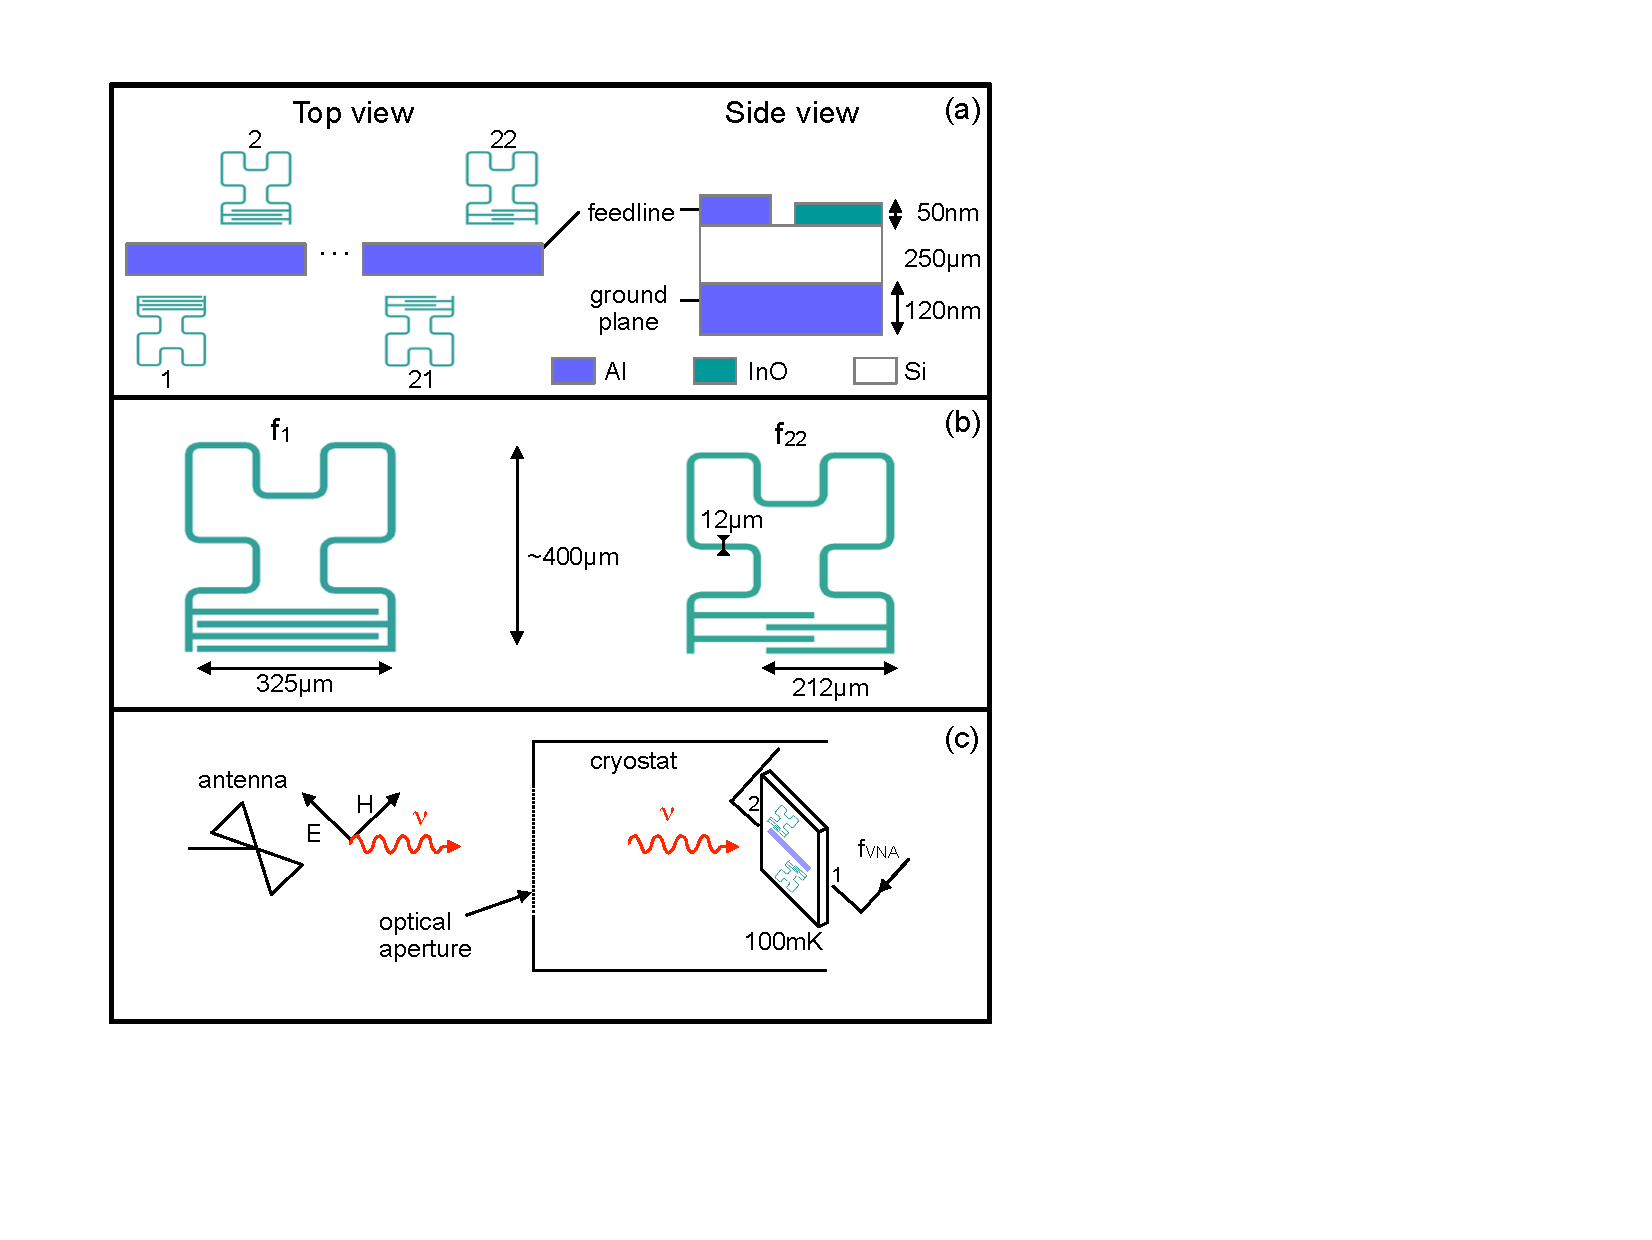
\includegraphics{fig/fig1}}
\caption{\textbf{ Experimental set-up.} (a) Resonators' design. Twenty-two resonators are capacitively coupled to the feedline. Cross-section view of the stripline configuration. (b) Detailed design of the $f_1$ and the $f_{22}$ resonators. The Hilbert fractal inductance is identical for all the resonators. The four capacitance fingers length are varied from one resonator to another : from the shortest for $f_{22}$ to the longest for $f_{1}$. (c) GHz-illumination sketch. A butterfly antenna at room temperature illuminates the resonators through optical apertures of the dilution fridge refrigerator. }
\label{design}
\end{center}
\end{figure}


Figure~\ref{design} displays the resonators design and a sketch of the experimental set-up. Twenty-two Indium Oxide resonators were deposited on a silicium substrate of 250$\mu$m. They are capacitively coupled to an aluminium transmission in a stripline configuration :  a feedline on the top of the substrate and a ground plane on the back. Each resonator consists of an Hilbert fractal inductance and of an interdigital capacitor. Frequency multiplexing is achieved by varying the capacitance using different fingers length. The design of the lowest ($f_1$)  and the higher frequency ($f_{22}$) resonators are detailled on figure~\ref{design}. The  $f_1$ and $f_{22}$ resonators correspond to a maximum total length of respectively 2.3~mm and 2.1~mm (from the first capacitor finger to the fourth one). The 50~nm Indium Oxyde film has a superconducting transition temperature $T_C$ of 2.8~K, a sheet inductance $L_S$ of 710~pH and a sheet resistance $R_S$ of 2000~$\Omega$. Sac\'ep\'e and collaborators~\cite{Sacepe} established by STM measurements that twice the superconducting gap of the employed Indium Oxyde worth about 200~GHz. The resonators were cooled down at 100~mK with a $^3$He/$^4$He dilution refrigerator. A butterfly antenna was placed at room temperature in front of the optical aperture of the cryostat to  illuminate the resonators in the GHz-range, see figure~\ref{design}(c).  A radio-frequency source was connected to the antenna and allowed to varied the GHz-illumination up to 20~GHz. The frequencies were monitored with a Vectorial Network Analyser (VNA) connected to the transmission line. 

%\section{Results}

\begin{figure}[h]
\begin{center}
\resizebox{8.5cm}{!}{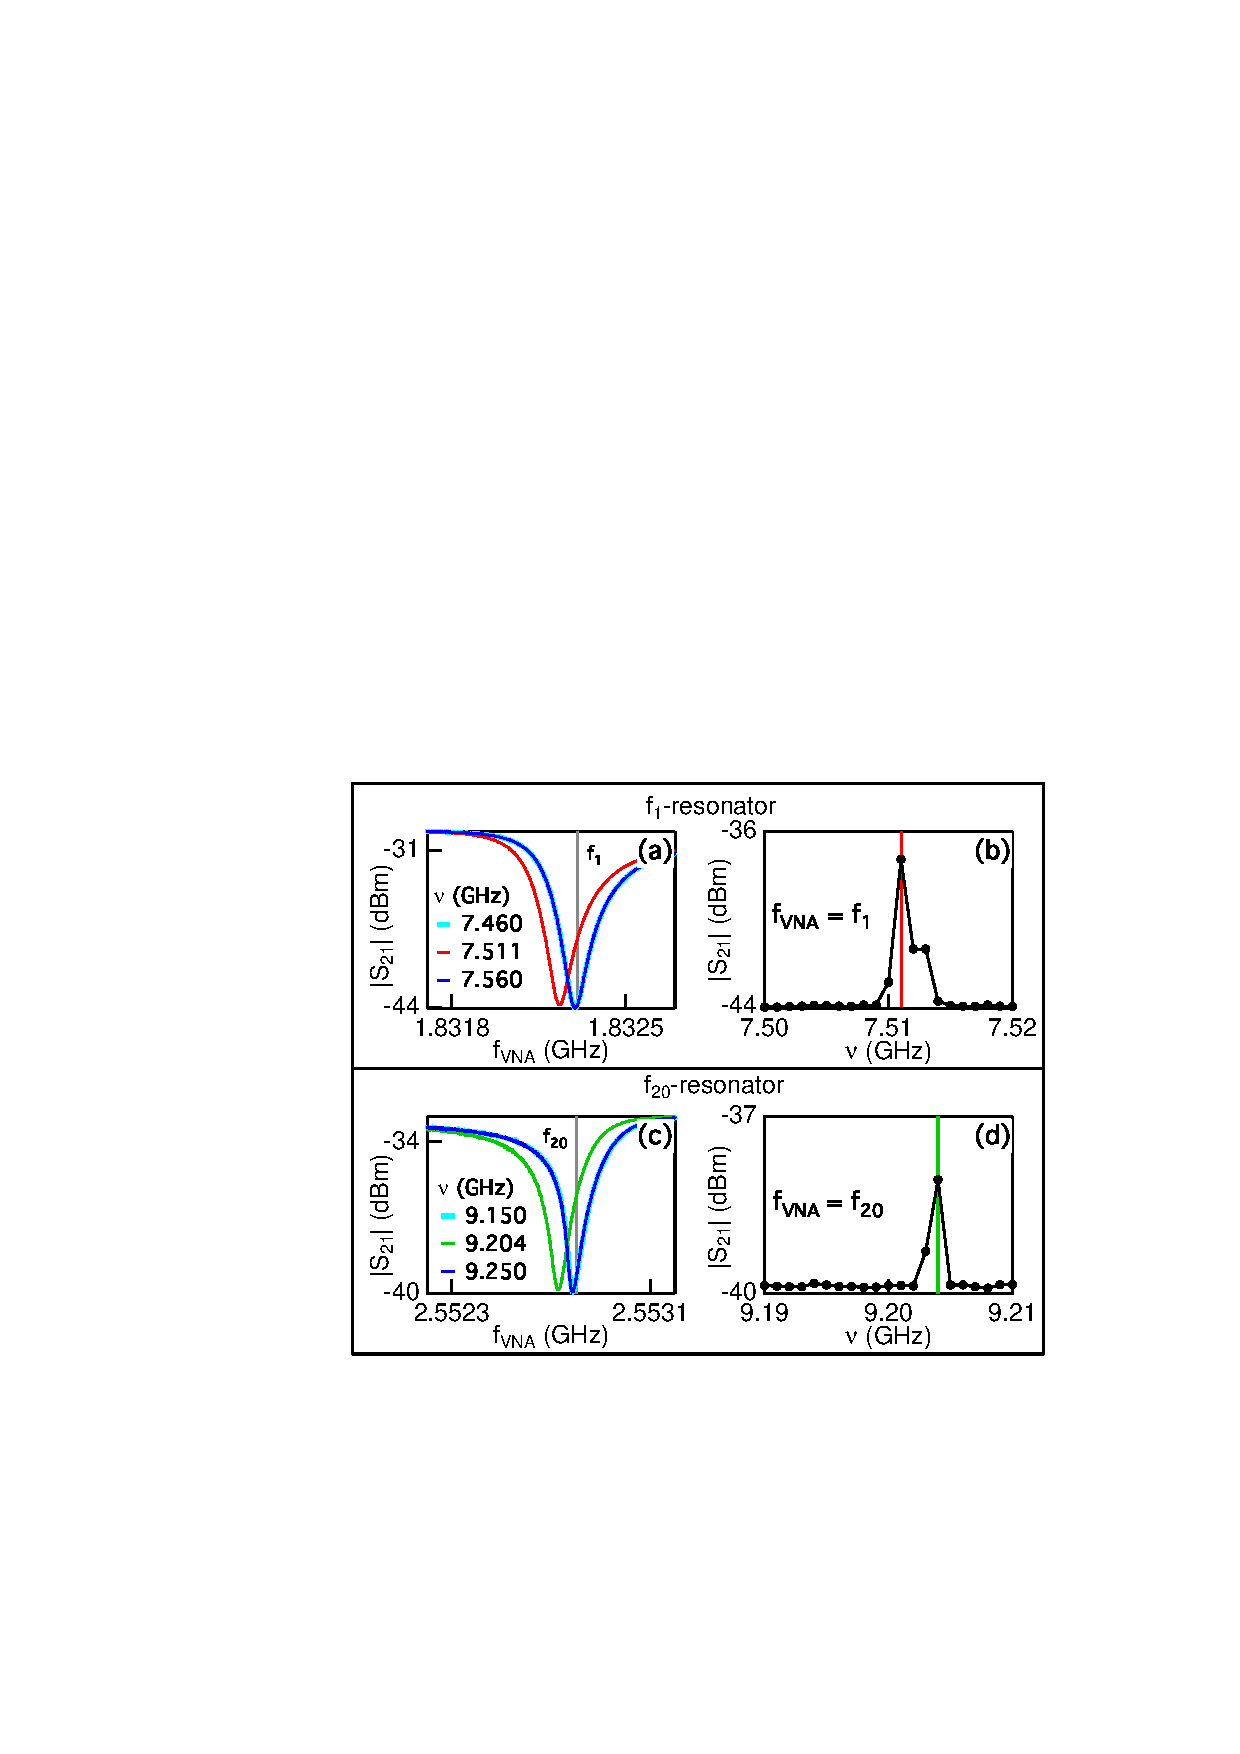
\includegraphics{fig/fig2}}
\caption{\textbf{VNA-measurements with a $\simeq$7-10~GHz-illumination.} (a),(b),(c) GHz-illumination energy scans at a fixed VNA-frequency : the unload $f$-frequencies. (d), (e) VNA-scans for various fixed GHz-illumination energy. (f) Light absorption frequency $w_{abs}$ as a function of the resonator number.}
\label{concept_tunabilty} 
\end{center}
\end{figure}

A large frequency vectorial network analyser scan revealed that 20 out of 22 resonators were functional. Figure~\ref{concept_tunabilty} depicts the results obtained for a $\simeq$7-10~GHz-illumination. Top panels (a) and (d) presents measurements realized on the $f_1$-resonator.  Middle panels (b) and (e) concern the $f_{20}$-resonator. The lowest panels gather measurements lead on different resonators. Two kind of VNA-measurements were performed: (a),(b),(c) are GHz-illumination energy scans realized at a fixed VNA-frequency: the unload $f$-frequencies (d), (e) are VNA-scans for various fixed GHz-illumination energy. The GHz-illumination energy scans presents a peak for each resonator. The peak correspond to light absorption  $\omega_{abs}$ that results in a shift of the resonance frequency as shown by the VNA-scans. Panel (f) displays the light absorption frequency $w_{abs}$ for each measured resonator as a function of the resonator number. This demonstrate that the light absorption frequency can be tuned with the total length of the superconducting resonator.


\begin{figure}[htbp]
\begin{center}
\resizebox{7cm}{!}{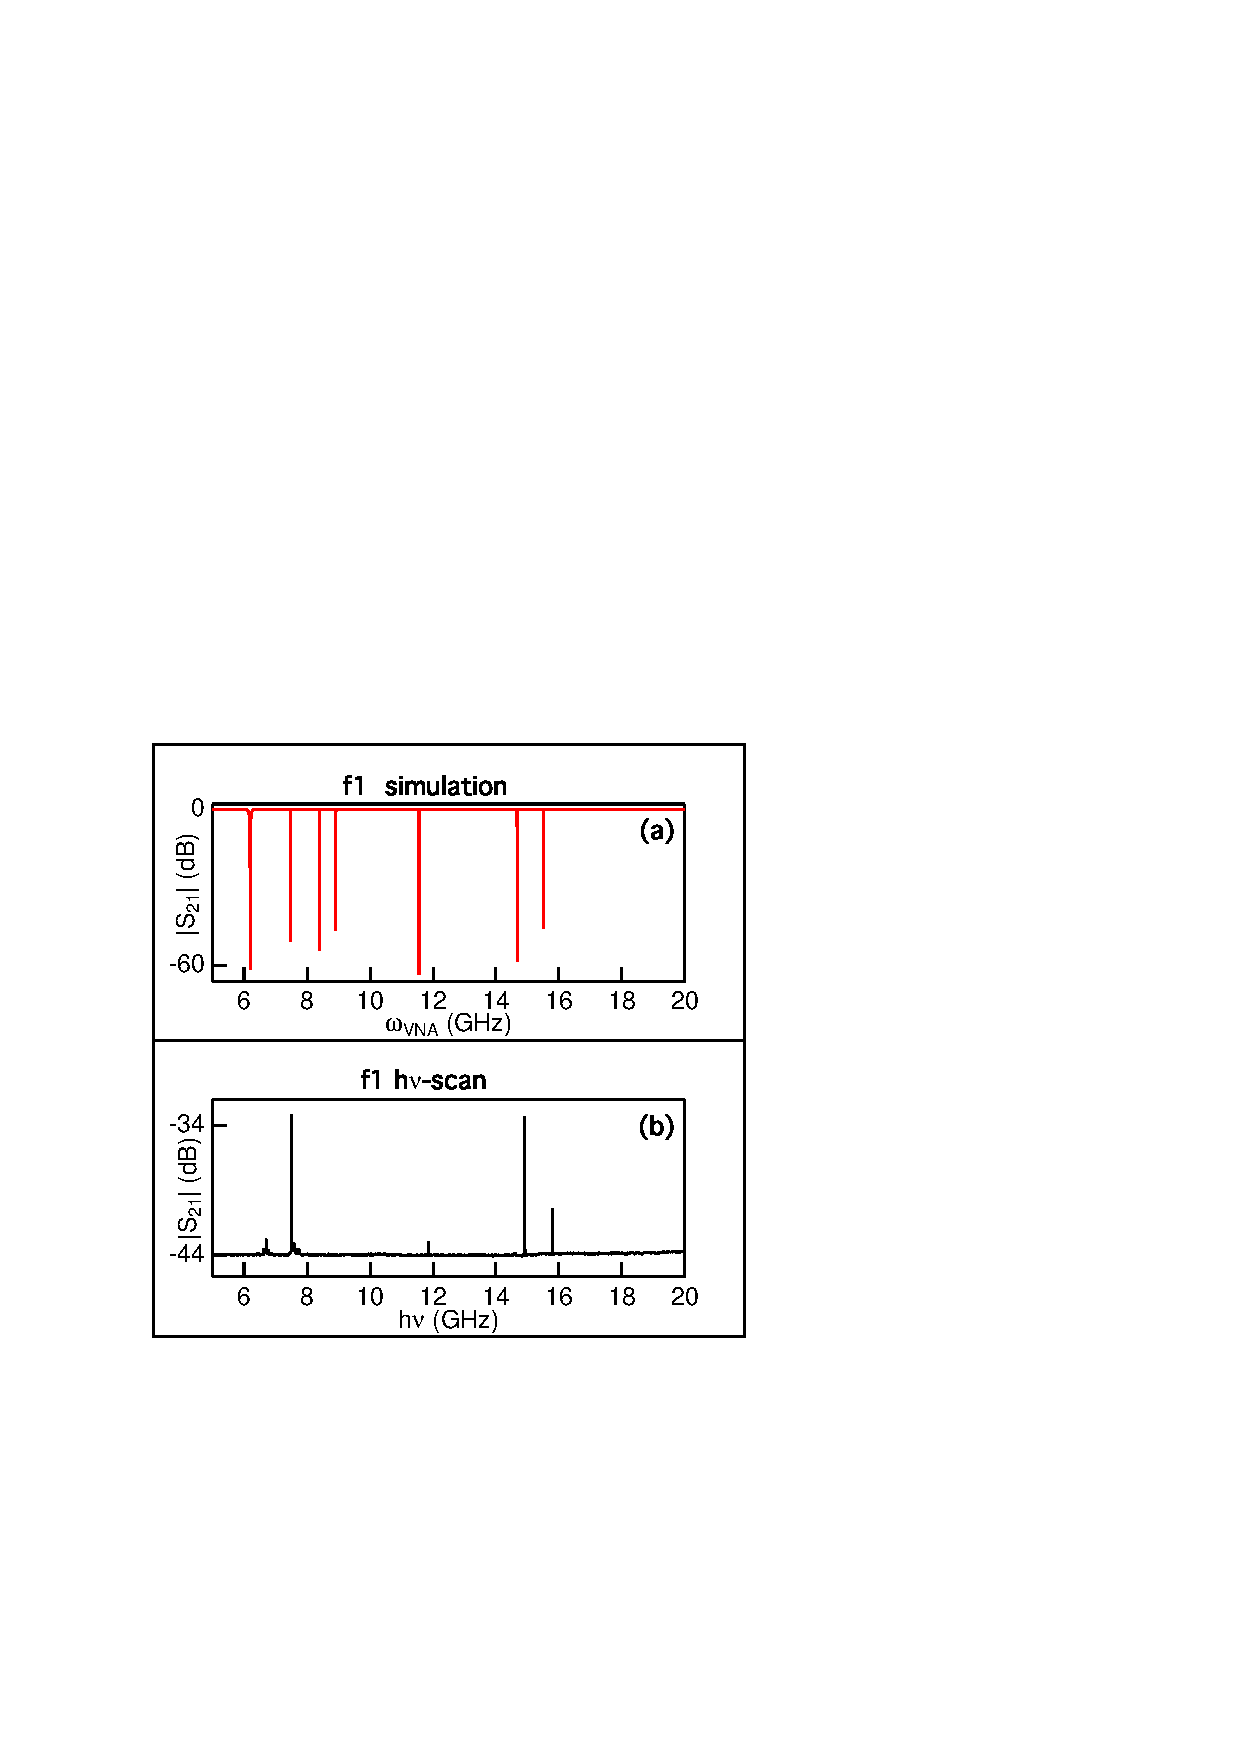
\includegraphics{fig/fig3}}
\caption{\textbf{Simulation and measurement on the f1-resonator.} (a) Simulation of $|S_{21}|$ as a function of the frequency for the $f_1$-resonator geometry. (b) Large bande GHz-illumination for a constante illumination power.}
\label{mult_abs}
\end{center}
\end{figure}


Figure~\ref{mult_abs} presents simulation and measurement realized on the $f_1$-resonator. The simulation has been done employing the SONNET software using for the aluminium transmission line: $R_{DC} = 1e^{-7}~\Omega/sq$, $L_S = 0.2~pH/sq$, for the silicium substrate: $d=250~\mu m$, $\epsilon_r=11.9$, for the in-out impedance $50~\Omega$ and for the indium oxyde material: $R_{DC} = 1e^{-6}~\Omega/sq$, $L_S = 710~pH/sq$. Within the 1-20~GHz range the simulation revealed eight resonances. The first harmonique, no shown on the figure, is the measured $f_1$-frequency. The sheet inductance of  indium oxyde has been adjusted to obtain the same $f_1$-frequency by simulation (1.80~GHz) and measurement (1.83~GHz), leading to a 1\% mismatch. Panel (b) presents the evolution of the  $|S_{21}(\omega_{VNA}=f_1)|$ magnitude as the illumination energy $h\nu$ is varied for a constant power (P=-25dB on the antenna). Different peaks are observed.  VNA-scans, as those presented on figure 2(d), confirmed that each observed peak corresponds to a shift of the resonance frequency. Two main peaks are observed at 7.51~GHz and 14.91~GHz with a energy selectivity lower than 0.04~GHz, demonstrating that the $f_1$-resonator is  sensitive to precise discrete light values within the GHz-range. Similar behavior as being observed for different resonators but for different $h\nu$ values. When observed light absorption frequencies match within 3\% with the computed resonance frequency as shown on table~\ref{tabwabs}. 

\begin{table}[h]
\caption{\textbf{Simulated and light absorption frequencies.} }
\begin{center}
\begin{tabular}{|c|c|c|}
\hline
$\omega_{sim}$ [GHz]&$\omega_{abs}$ [GHz] &error [\%] \\
\hline
6.20&x&x\\
7.47&7.51&1\\
8.41&x&x\\
8.92&x&x\\
11.56&11.86&3\\
14.67&14.91&2\\
15.51&15.81&2\\
\hline
\end{tabular}
\label{tabwabs}
\end{center}

\end{table}


%decrire fig4= �tude puissance et polarisation
%discussion pas de changement de factuer de qualit�


Figure~\ref{power_polar_Qfactor} shows VNA-measurements on the $f_{1}$ and $f_{20}$ resonators. Panels (a) and (c) demonstrate that the frequency shift due the 7-10~GHz light absorption increases with the incident power above a threshold. The power indicated correspond to the power apply onto the antenna with the RF-source. The power threshold worth, respectively for $f_{1}$ and $f_{20}$, -50~dB and -35~dB. The corresponding incident power onto the detector was estimated to be respectively  XX dB and XXdB. Panels (b) and (d) tend to indicate that the polarization affects the light absorption. The polarization rules selections differ between the two 
resonators. The angle indicates the orientation between the feedline and the light electric field (that is the longer direction of the butterfly antenna). It worth to notice that the incident light also carries a magnetic field that is  perpendicular to the electric field. From the measurements presented it is not possible to conclude wether the electric or the magnetic field orientation is relevant  for the mechanism at play.

\begin{figure}[htbp]
\begin{center}
\resizebox{8.5cm}{!}{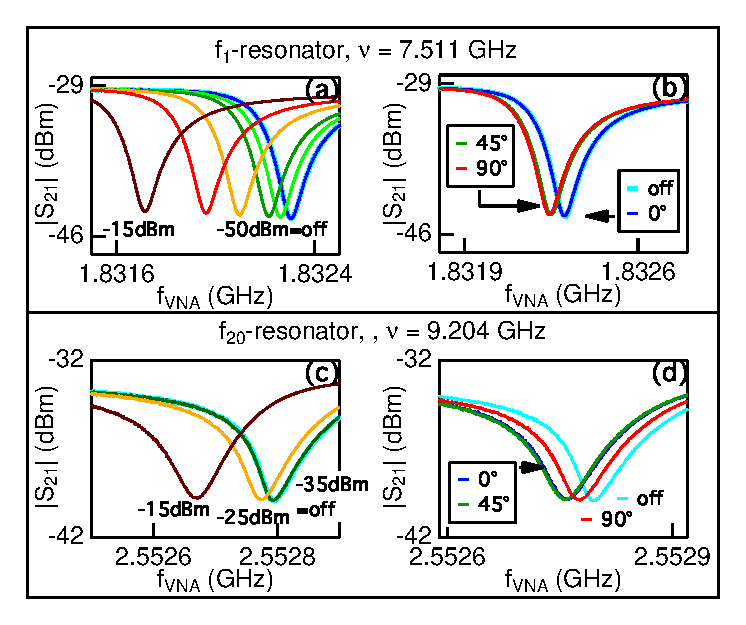
\includegraphics{fig/fig4}}
\caption{\textbf{Power and polarization studies.} (a), (c) Power illumination influence. Power apply on the antenna is, from right to left, in dB : (a) off, -50, -45, -35, -25,- 20, -15 (b) off, -35, -25, -15. (b), (d) Polarization study. Angles indicate the orientation between the light electric field and the feedline. }
\label{power_polar_Qfactor}
\end{center}
\end{figure}

%\section{Discussion}
%definition

We attributed our observations to surface superconducting plasmons. A superconducting surface plasmon is a collective oscillation of the superfluid paired electrons that propagates at the interface between the superconductor and a dielectric medium. This mode is confined in the direction perpendicular to the interface. It is a transverse magnetic polarized mode. In granular aluminum superconducting film deposited on SrTiO$_3$ (a high dielectric constant material), the following plasmons surface dispersion law has been evidence~\cite{Buisson}:

\begin{equation}
\omega_p^2=\frac{n_se^2}{m\epsilon_0\epsilon_r}k=\frac{n_se^2}{m\epsilon_0\epsilon_r}\frac{n\pi}{a}
\label{plasmon_2D}
\end{equation}

\noindent where $n_s$ is the surface superfluid density, $\epsilon_r$ the relative dielectric constant of the substrate and $k$ the propagation vector that satisfies $k = n\pi/a$ where a is the length of the film and n an integer. From equation~(\ref{plasmon_2D}) it is clear that low surface superfluid density, as anticipated for Indium Oxyde, will contribute to lower the plasmon frequency below twice the superconducting gap. 


%estimation ns

To estimate the surface superfluid density of our Indium Oxyde material we employed two different methods. For the first method we simply consider the superfluid density to be inversely proportional to the resistance per square. We used from reference~\cite{Buisson}: $n_s(AlO_x)~=~2\times10^{16}~m^{-2}$ and $R(AlO_x)~=~300~\Omega/sq$, and, for our material $R(InO_x)~=~2000~\Omega/sq$. We obtained $n_s(InO_x)~=~3\times10^{15}~m^{-2}$. Doing this, we implicitly assumed that the quasiparticle lifetime $\tau_{qp}$ in both materials are very similar. The second method estimates the surface superfluid density from the kinetic inductance $L_s$ using:

\begin{equation}
n_s=\frac{m}{L_se^2}(1+\frac{\xi_0}{l})
\label{ns_ls}
\end{equation}

\noindent where $\xi_0$ is the superconducting coherence length and l is the mean free path. In the clean limit, when $\xi_0/l\rightarrow0$, we get the lower limit value of the surface superfluid density $n_s(InO_x)~=~3.85\times10^{14}~m^{-2}$. From references~\cite{reffff} we can estimate $\xi_0/l\simeq10-20$ resulting in  $n_s(InO_x)~=~3.85\times10^{15}-7.7\times10^{15}~m^{-2}$. Eventually using  equation~(\ref{plasmon_2D}) with n$_s$ =4.2$\times$10$^{15}$ m$^{-2}$, $\epsilon_r$=11.9 (silicium substrate), n=1, a=2.3~mm (length of the $f_1$ resonator from the first capacitor finger to the fourth one) we get a surface plasmon frequency of 6.23~GHz corresponding to the  6.20~GHz harmonique simulated using the SONNET software, see table~\ref{tabwabs}. 

The observed light absorption can be interpreted in term of higher harmonique plasmons, corresponding in equation~(\ref{plasmon_2D}) to n=2, 3, etc... However, as the geometry of our resonators differ from a planar thin film more complex resonating modes are realized as revealed  by simulation, cf table~\ref{tabwabs}. The difference of polarization rule selection between the $f_1$ and the $f_{20}$ resonators evidence on figure~\ref{power_polar_Qfactor} might be due to a change of  resonating mode type (as suggested by simulations of current distribution). Up to date, we are not able to explain why some modes are more light sensitive than others.

A surface plasmon mechanism accounts for the shifted of the fondamental resonance frequency through absorption of very precise light radiation frequencies. Indeed, in order to be absorbed the light radiation has to match a surface plasmon frequency, and, when absorbed the inductance of the resonator is modified through nodes created by the plasmon oscillation. The mechanism also explains why the light absorption frequency varies with the resonator length. 

%\begin{figure*}[htbp]
%\begin{center}
%\resizebox{17cm}{!}{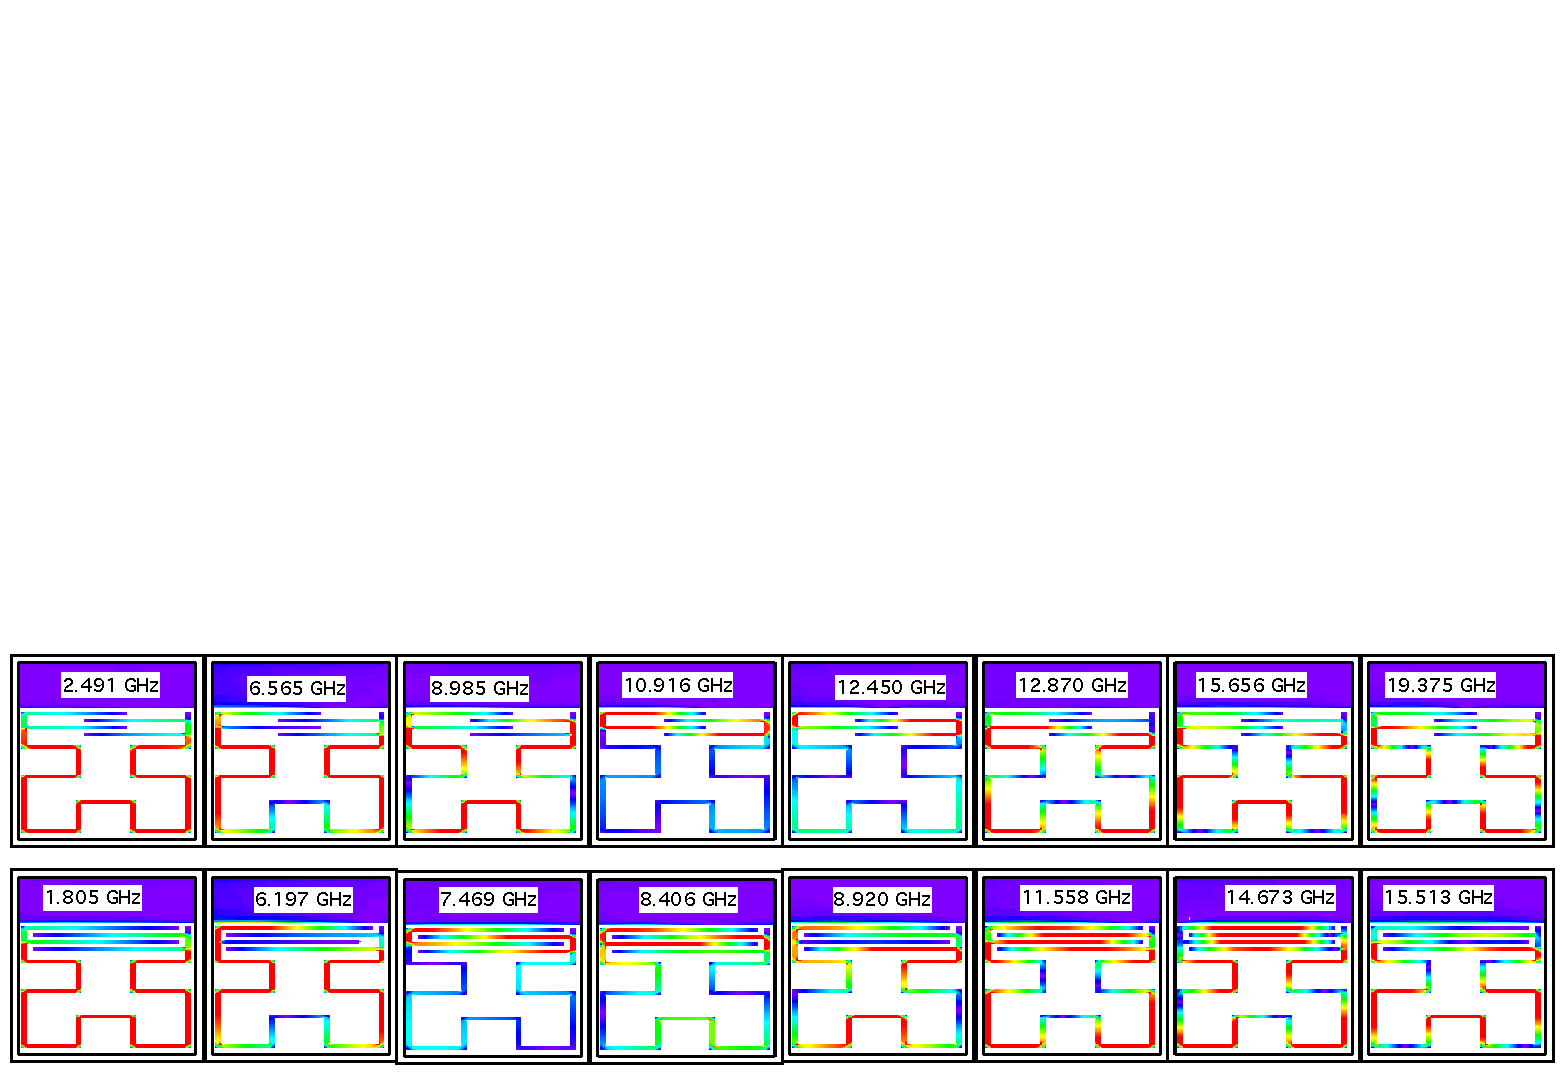
\includegraphics{fig/fig5}}
%\caption{\textbf{ Simulations of the courant distribution}}
%\label{SONNET}
%\end{center}
%\end{figure*}
As butterfly antenna already detects centimetric radiation it is legitimate to address the question of our detection technique interest.  First, thanks to multiplexing, matrix of detectors can be envisioned. Second, high energy selectivity is possible. Third, the sensitivity may be factor of magnitude higher because of the large quality factor. Eventually, extension to lower radiation detection of experiment already enclosing KIDs would be ease thanks to cryogenic and electronic readout compatibility.



%\section{Conclusion}
In conclusion, we have realized the first functional Indium Oxide superconducting resonators. We demonstrated that they are sensitive to sub-gap radiations with precise discrete values that can can be tuned with the length of the superconducting resonator. We explained those observations within a surface plasmon mechanism. 

\vspace{0.5cm}
%\section*{Acknowledgments}
We acknowledge M. Feigelman for directing us towards superconducting surface plasmons and O. Buisson for useful discussions. This work is supported by the French National Research Agency through Grant No. ANR-12-JS04-0003-01 SUBRISSYME.

\bibliographystyle{unsrt}
\begin{thebibliography}{99}
\bibitem{Day} P. K. Day and al, Nature 425,  817 (2003). 
\bibitem{Wallraff} A. Wallraff and al, Nature 431, 162 (2004). 
\bibitem{Regal} C. A. Regal and al, Nature Physics 4, 555 (2008). 
\bibitem{Sacepe} B. Sac\'ep\'e and al, 
\bibitem{Buisson} O. Buisson and al, Physical Review Letters 73, 3153 (1994).
\bibitem{Buisson1D} O. Buisson and al, Physical Review Letters 86, 3 (2000).

\end{thebibliography}



 \end{document}